\section{Artefact Design}
\label{sec:artefact}

This section gives a factual description of the artefact as built: its requirements (Table~\ref{tab:spec}) and its architecture (Figure~\ref{fig:arch}).

\subsection{Design Specifications}

\begin{table}[ht]
\centering\small
\caption{Design specification: functional (F) and non-functional (N) requirements}
\label{tab:spec}
\begin{tabularx}{\linewidth}{lYl}
\toprule
\textbf{ID} & \textbf{Requirement} & \textbf{Obj.}\\
\midrule
F1 & Accept a JPEG/PNG face photo up to 10\,MB from camera or gallery & O5\\
F2 & Reject images without a detectable face and explain how to retake the photo & O5\\
F3 & Return a score, threshold and status (\emph{present}, \emph{absent} or \emph{uncertain}) for each of five concerns & O2\\
F4 & Accept an optional user skin type (dry, normal, oily, combination, sensitive); never infer it from the photo & O4\\
F5 & Recommend up to five products per relevant category, with the matched ingredients and a score & O4\\
F6 & Suggest a morning and evening routine derived from the detected concerns & O4\\
F7 & Browse, search, filter and sort the catalogue; view product detail; save favourites & O5\\
F8 & Keep a local history of past checks & O5\\
F9 & Answer free-text questions through a grounded chat assistant, falling back to rules if the language model is unavailable & O5\\
F10 & Show a non-medical disclaimer on every result and chat screen & O5\\
\midrule
N1 & No medical labels; wording must describe observations, not diagnoses & --\\
N2 & Thresholds are set on validation data only; the test set is used only for reporting & O2\\
N3 & Photos are not stored on the server; history is kept on the device only & --\\
N4 & Warm analysis completes in under 2 seconds on a laptop CPU & O5\\
N5 & Runs entirely on free, open-source software without paid APIs & --\\
N6 & Structured API errors (400/404/422/500) so the client can show helpful messages & O5\\
\bottomrule
\end{tabularx}
\end{table}

\subsection{Artefact's Structure/ Architecture / Framework}

\subsubsection*{Architectural style}

SkinCare AI uses a \textbf{three-tier client--server architecture} (Figure~\ref{fig:arch}):
\begin{enumerate}
  \item a \emph{presentation tier}, the Expo/React Native mobile client;
  \item an \emph{application tier}, a stateless FastAPI REST service that holds the model, face gate, recommender and language model in memory;
  \item a \emph{data tier} of read-only files: model weights and thresholds, the product catalogue and the ingredient mappings.
\end{enumerate}

Three design principles shape this structure:
\begin{itemize}
  \item \textbf{Separation of concerns.} The client only collects input and displays results. All analysis and ranking happens on the server, so the model can be replaced without changing the app.
  \item \textbf{Statelessness and privacy by design.} The server stores no photos and no user data. Each request carries everything needed to answer it, and history and favourites are kept only on the device (requirement N3).
  \item \textbf{Graceful degradation.} The language model is optional. If it is unavailable, slow or returns invalid output, a deterministic rule-based answer is used, so the core photo-to-product flow never depends on it.
\end{itemize}

\begin{figure}[p]
\centering
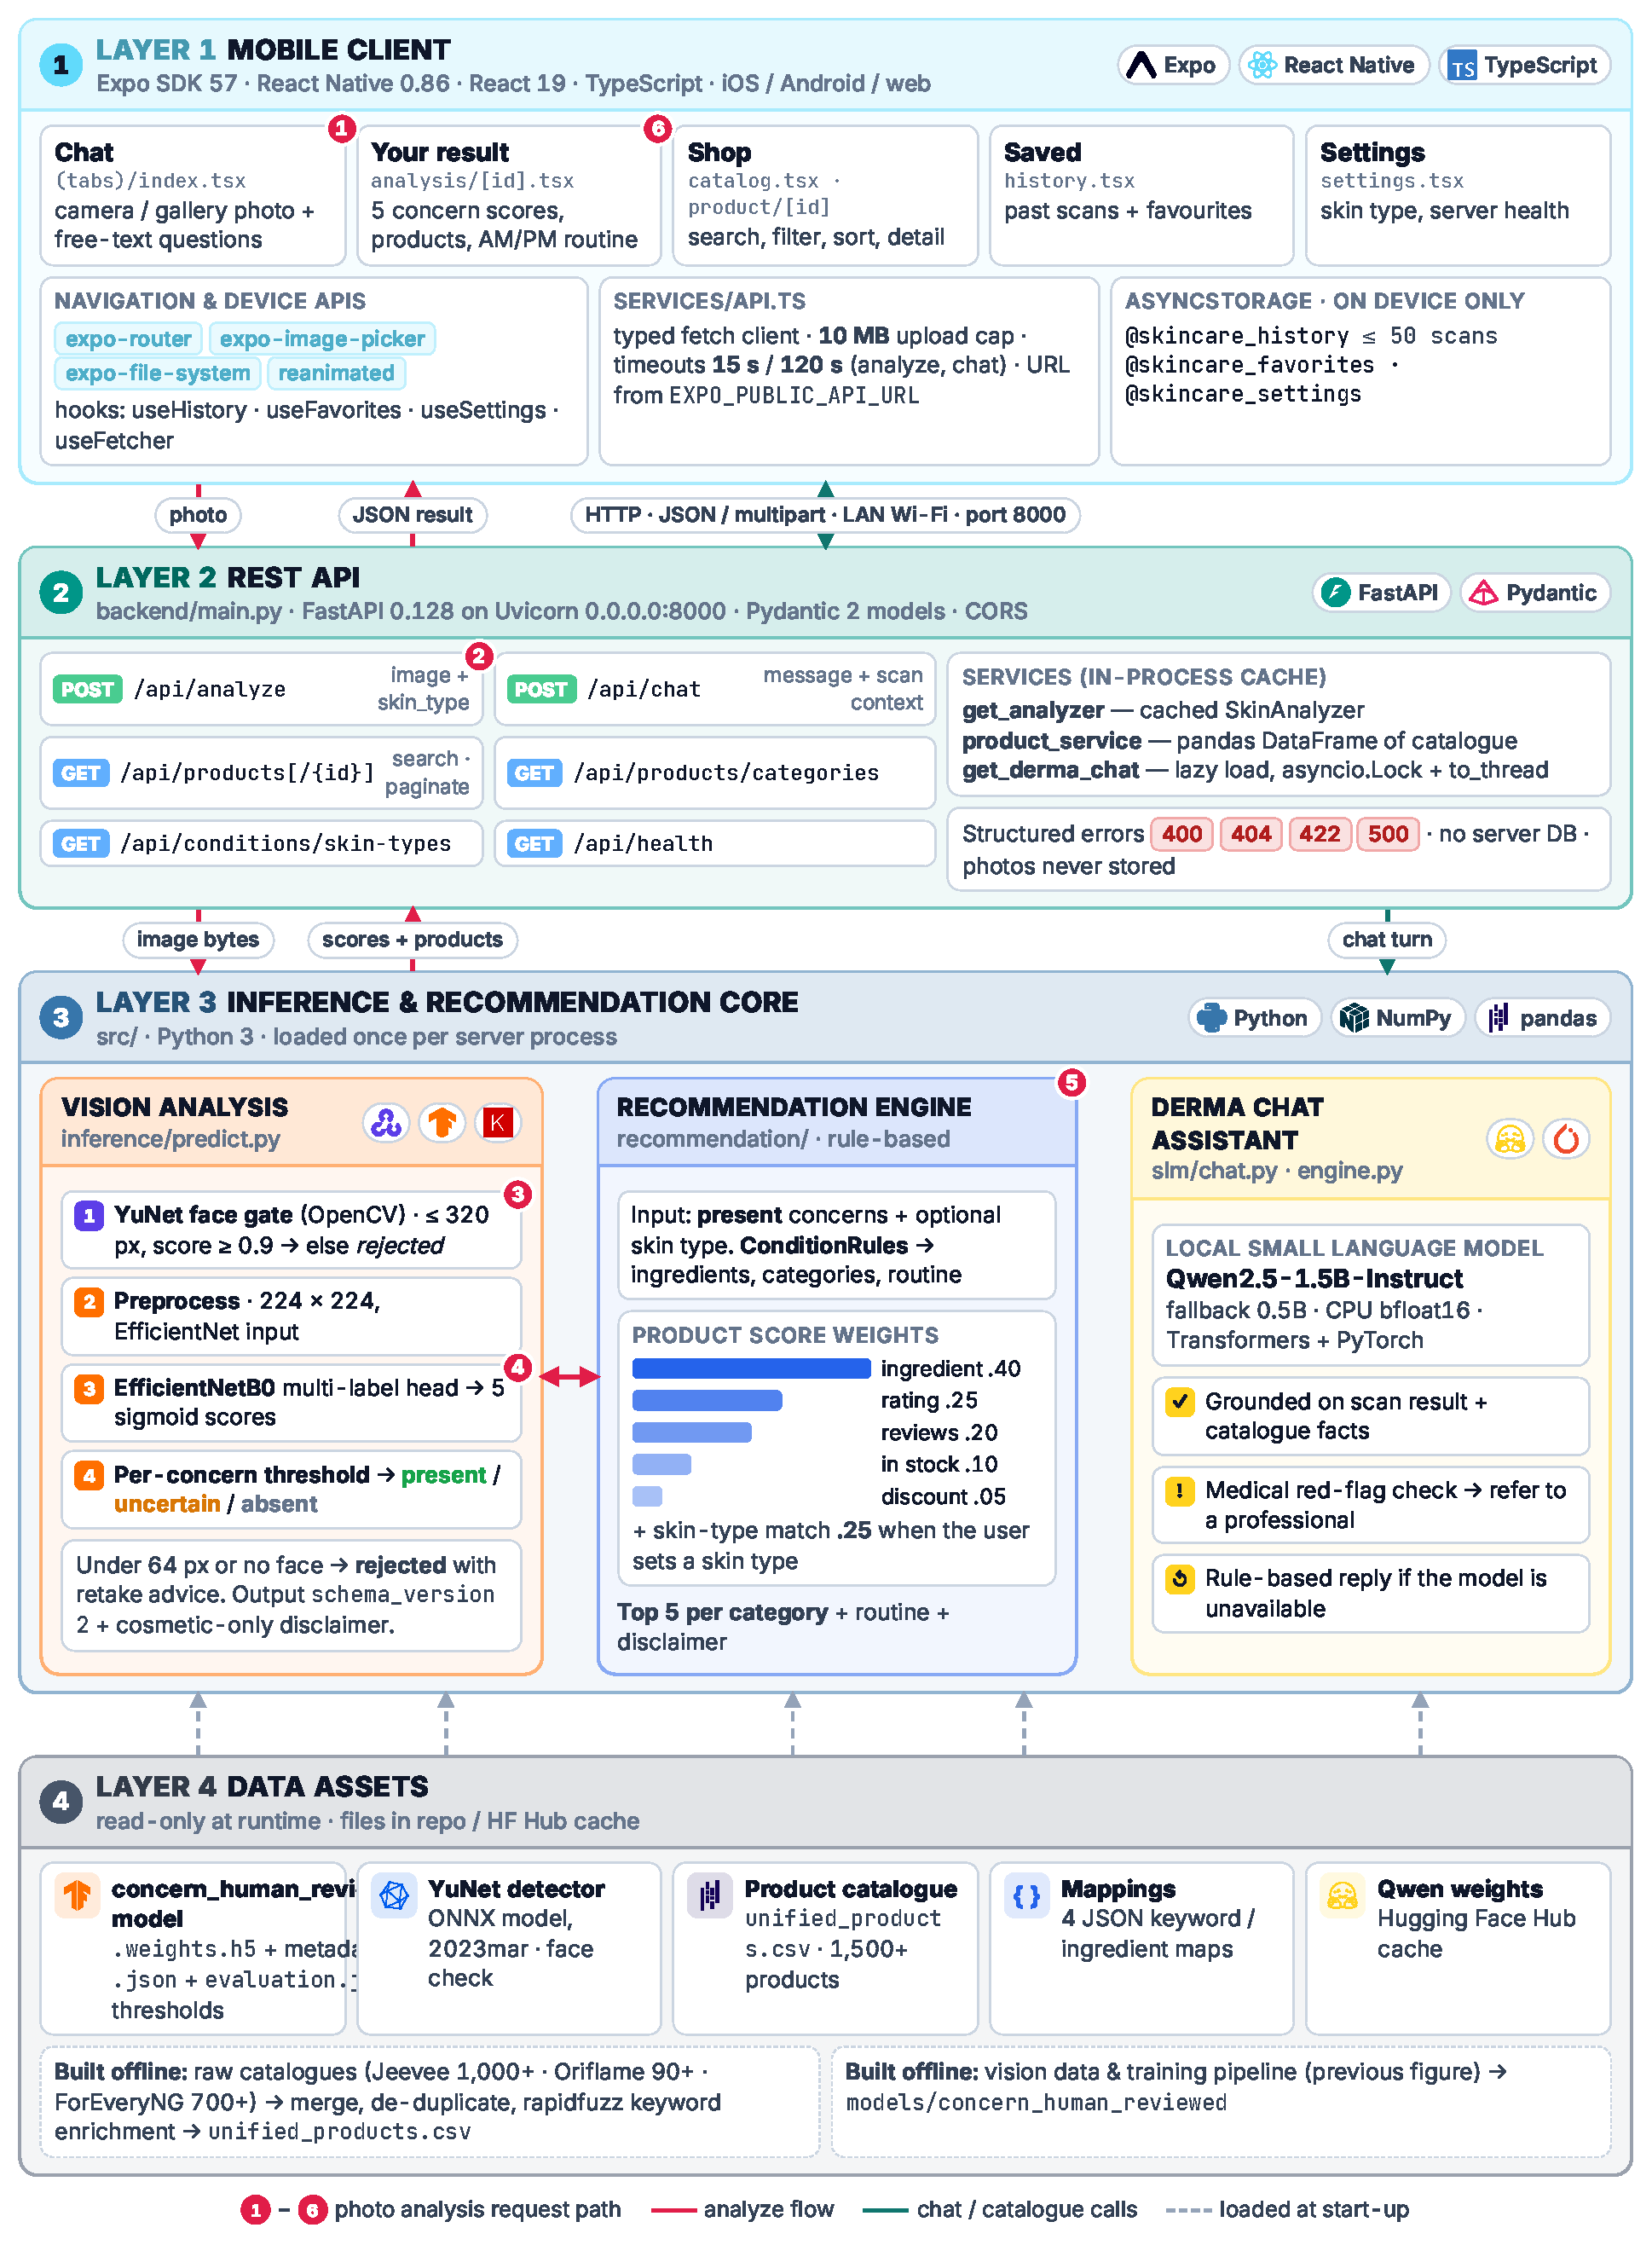
\includegraphics[width=\linewidth]{figures/architecture.pdf}
\caption{System architecture of SkinCare AI: Expo/React Native client, FastAPI layer, Python inference and recommendation core (TensorFlow, OpenCV, Transformers), and data assets}
\label{fig:arch}
\end{figure}

\subsubsection*{Components}

Table~\ref{tab:components} lists the main components, what each is responsible for and where it lives in the code.

\begin{table}[ht]
\centering\small
\caption{Main components of the artefact}
\label{tab:components}
\begin{tabularx}{\linewidth}{P{2.6cm}YP{4.3cm}}
\toprule
\textbf{Component} & \textbf{Responsibility} & \textbf{Implementation}\\
\midrule
Mobile client & Tabs for Chat, Shop, Saved and Settings; photo capture; result, routine and product screens; on-device history and favourites & \texttt{mobile/app}, \texttt{mobile/services/api.ts}, AsyncStorage hooks\\
API layer & Validates uploads and parameters, routes requests, returns structured errors (400/404/422/500) & FastAPI routers in \texttt{backend/routes}\\
Face gate & Rejects photos without a clear face (YuNet score $\geq 0.9$) & \texttt{SkinAnalyzer} with OpenCV \texttt{FaceDetectorYN}\\
Concern model & Shared preprocessing, five sigmoid scores, per-concern thresholds and status & \texttt{SkinAnalyzer} in \texttt{predict.py}; shared \texttt{concern\_\allowbreak preprocessing.py}\\
Recommender & Maps present concerns to ingredients and categories; ranks products by weighted score & \texttt{RecommendationEngine}, \texttt{ConditionRules}, \texttt{scoring.py}\\
Language-model layer & Optional re-ranking and grounded chat; rule-based fallback; red-flag signposting & \texttt{SlmEngine}, \texttt{DermaChat}, \texttt{SlmRecommender} (Qwen2.5)\\
Data assets & Model weights, \texttt{evaluation.json} thresholds, product catalogue, ingredient mappings & \texttt{models/}, \texttt{data/enriched}, \texttt{data/mappings}\\
\bottomrule
\end{tabularx}
\end{table}

\subsubsection*{API interface}

The client and server communicate only through the REST endpoints in Table~\ref{tab:api}. Analysis responses carry a schema version, the model version and the disclaimer, and their structure is fixed by a contract unit test.

\begin{table}[ht]
\centering\small
\caption{REST API endpoints}
\label{tab:api}
\begin{tabularx}{\linewidth}{lP{4.9cm}Y}
\toprule
\textbf{Method} & \textbf{Path} & \textbf{Purpose}\\
\midrule
GET & \texttt{/api/health} & Connection check used by the app's ``Test connection'' button\\
POST & \texttt{/api/analyze} & Multipart photo plus optional skin type; returns concerns, routine and recommendations\\
POST & \texttt{/api/chat} & Question plus optional latest result; returns a grounded reply and product cards\\
GET & \texttt{/api/products} & Catalogue search, filter by category and skin type, sort and paginate\\
GET & \texttt{/api/products/categories} & List of product categories\\
GET & \texttt{/api/products/\{id\}} & Product detail, or 404\\
GET & \texttt{/api/conditions/skin-types} & The five skin types with recommended ingredients\\
\bottomrule
\end{tabularx}
\end{table}

\subsubsection*{Analysis request flow}

When the client uploads a photo to \texttt{/api/analyze}, the server processes it in five steps:
\begin{enumerate}
  \item It checks the MIME type and size of the upload.
  \item It decodes the image to RGB and runs YuNet on a copy resized to at most 320\,px. If no face scores at least 0.9, it returns a \emph{rejected} result that explains how to retake the photo.
  \item It preprocesses the image exactly as during training: bilinear resize to 224$\times$224 followed by EfficientNet normalisation. This code is shared by training, evaluation and serving.
  \item It predicts five sigmoid scores. A score within $\pm0.05$ of its concern's threshold is labelled \emph{uncertain}, a higher score \emph{present}, and a lower score \emph{absent}.
  \item It passes the concerns marked \emph{present}, and the stated skin type, to the recommender, and returns the combined result.
\end{enumerate}

\subsubsection*{Core modules}

\textbf{Model.} The network is EfficientNetB0 without its ImageNet head, followed by global average pooling, dropout (0.3), a 128-unit ReLU layer and a 5-unit sigmoid output. It has about 4.2 million parameters in total. Per-concern thresholds are loaded from the model's \texttt{evaluation.json} file, so re-evaluating the model updates the live app without any code change.

\label{sec:recommender}
\textbf{Recommender.} Table~\ref{tab:rules} lists the rule map. For each category relevant to the present concerns, every product in that category receives a score:
\begin{equation}
s = w_i\,I + w_r\,\tfrac{\text{rating}}{5} + w_v\,\tfrac{\log(1+\text{reviews})}{\log 1001} + w_a\,\mathbf{1}[\text{in stock}] + w_d\,\min(2\cdot\text{discount},1) + w_t\,T
\end{equation}
Here $I$ is the fraction of target ingredients that the product contains, and $T$ is its match to the stated skin type. The weights are $(w_i,w_r,w_v,w_a,w_d,w_t) = (0.40,0.25,0.20,0.10,0.05,0)$ when no skin type is given, and $(0.35,0.20,0.12,0.06,0.02,0.25)$ when one is. The top five products per category are returned together with the ingredients they matched. If no concern is present, a basic cleanser, moisturiser and sunscreen routine is suggested.

\begin{table}[ht]
\centering\small
\caption{Concern-to-ingredient and category rules used by the recommender}
\label{tab:rules}
\begin{tabularx}{\linewidth}{lYY}
\toprule
\textbf{Concern} & \textbf{Target ingredients} & \textbf{Categories}\\
\midrule
Blemishes & salicylic acid, niacinamide, tea tree, zinc, glycolic acid & cleanser, serum, moisturiser, spot treatment, toner\\
Dark spots & vitamin C, niacinamide, kojic acid, arbutin, glycolic acid, azelaic acid & cleanser, serum, moisturiser, spot treatment, sunscreen\\
Redness & centella asiatica, ceramides, aloe vera, niacinamide, panthenol & cleanser, moisturiser, sunscreen, serum\\
Visible pores & niacinamide, salicylic acid, zinc, glycolic acid & cleanser, toner, serum, moisturiser\\
Fine lines & retinol, hyaluronic acid, peptides, ceramides, vitamin C & cleanser, serum, moisturiser, sunscreen\\
\bottomrule
\end{tabularx}
\end{table}

\textbf{Language-model layer.} \texttt{Qwen2.5-1.5B-Instruct}, with a \texttt{0.5B} fallback, runs on the CPU. It is used in two places:
\begin{itemize}
  \item optionally, to reorder and justify the top candidates in an analysis result;
  \item for the chat assistant.
\end{itemize}
The prompt contains only catalogue facts for the candidate products. The response is parsed as JSON, and any product ID not in the candidate list is discarded in code. If the model is unavailable, or produces nothing valid, a deterministic rule-based answer is returned instead.

\textbf{Technology stack.} Table~\ref{tab:stack} summarises the stack.

\begin{table}[ht]
\centering\small
\caption{Technology stack}
\label{tab:stack}
\begin{tabularx}{\linewidth}{lY}
\toprule
\textbf{Layer} & \textbf{Technologies}\\
\midrule
Model \& data & Python 3.9, TensorFlow 2.16 / Keras, OpenCV (YuNet), pandas, NumPy, rapidfuzz, Pillow\\
Backend & FastAPI, Uvicorn, Pydantic, Hugging Face Transformers (Qwen2.5)\\
Mobile & Expo SDK, React Native, expo-router, TypeScript, AsyncStorage, expo-image-picker\\
Tooling & Streamlit (annotation and demonstration), Git, unittest\\
\bottomrule
\end{tabularx}
\end{table}
